
\subsection{Data science process}
There are many different lifecycle models to describe phases in a data science project. This section will give a quick overview of some important ones.

We'll start with \textbf{CRISP-DM}\sidenote{CRISP-DM} which stands for "Cross-industry standard process for data mining". It was developed in the late 1990s by different involved companies (SPSS, Teradata, Daimler AG, NCR Corporation, Ohra). The process consists of multiple steps playing together as visualized in \ref{fig:1_crisp_dm}

\begin{figure}[H]
  \centering
  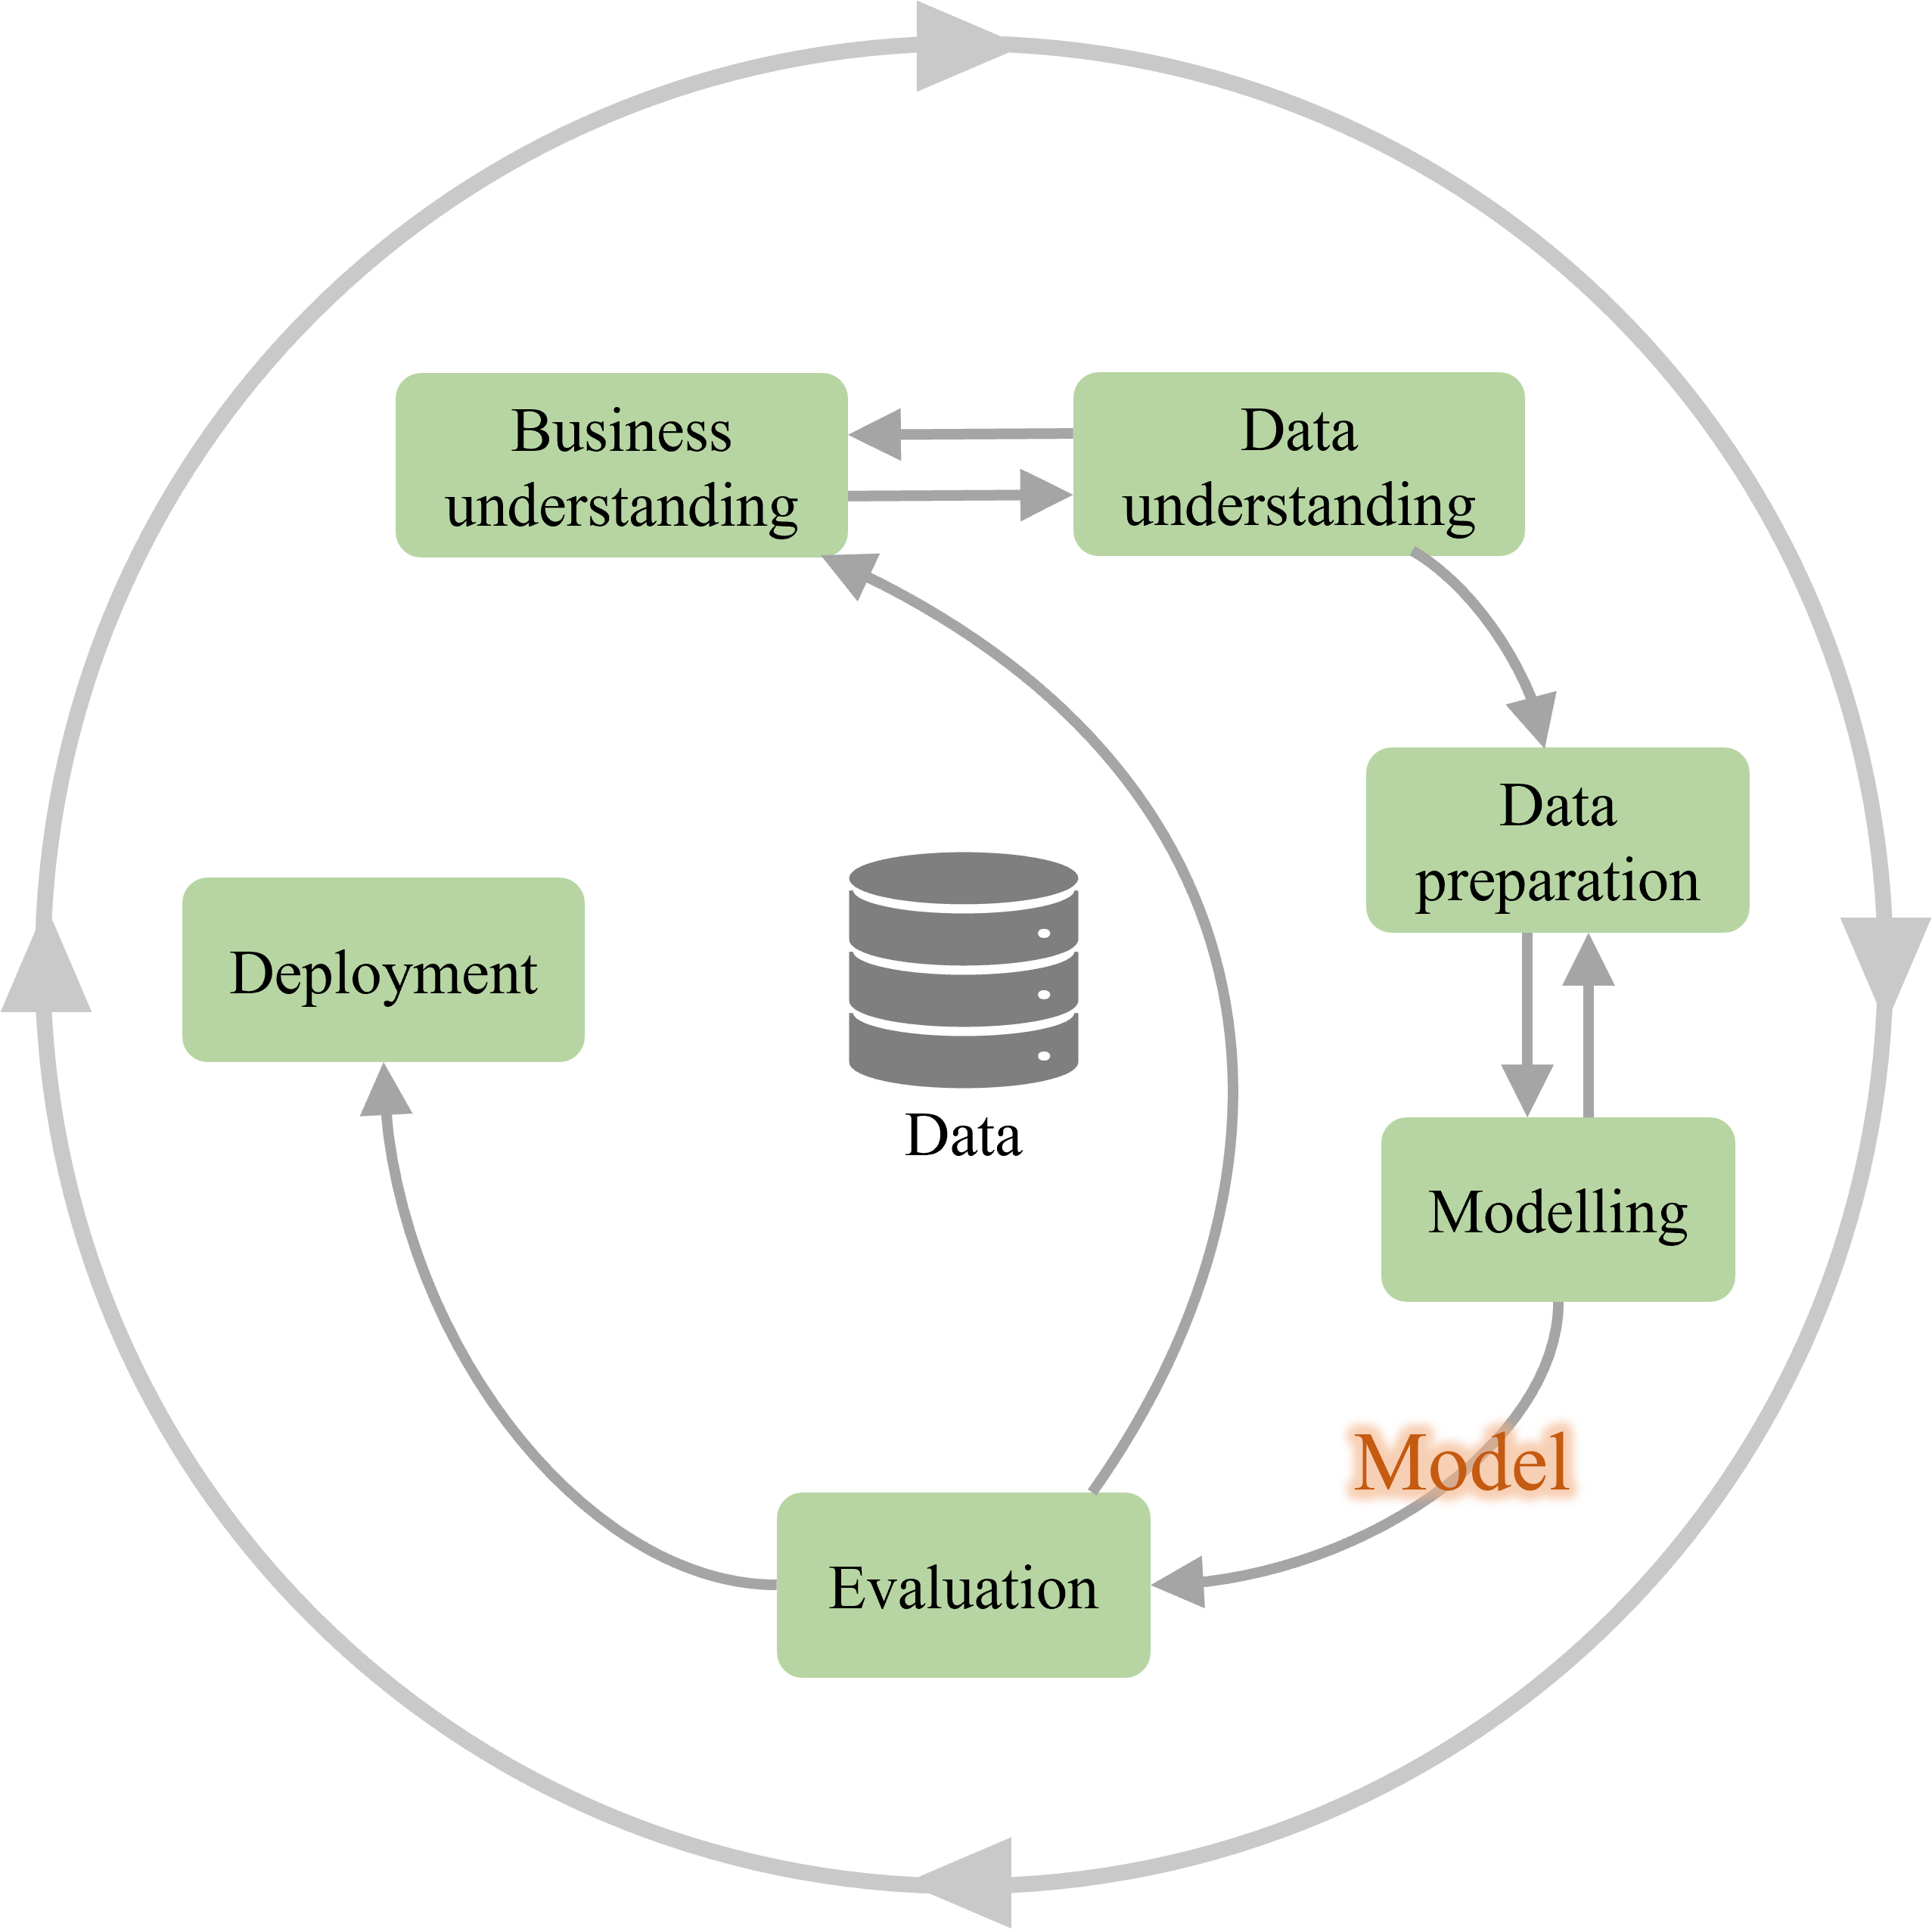
\includegraphics[width=0.5\textwidth]{assets/basics/crisp-dm.png}
  \caption{CRISP-DM process}
  \label{fig:1_crisp_dm}
\end{figure}

\begin{longtable}{p{0.0025\linewidth} >{\color{black}}p{0.35\linewidth} >{\color{gray}\footnotesize}p{0.6475\linewidth}}
  \multicolumn{3}{l}{\textbf{Business understanding}} \\
  & Determine business objective & Background, business objective, business success criteria \\
  & Situation assessment & Inventory of resources, requirements, assumptions, constraints, risks, contingencies, terminology, costs, benefits \\
  & Determine data mining goal & Data mining goals, data mining success criteria \\
  & Produce project plan & Project plan, initial assessment of tools and techniques \\[5pt]
  
  \multicolumn{3}{l}{\textbf{Data understanding}} \\
  & Collect initial data & Initial data collection report \\
  & Describe and explore data & Data description, exploration report \\
  & Verify data quality & Data quality report \\[5pt]
  
  \multicolumn{3}{l}{\textbf{Data preparation}} \\
  & Starting point: data set & Data set, data set description \\
  & Select data & Rationale for inclusion and exclusion \\
  & Clean data & Data cleaning report \\
  & Construct data & Derived attributes, generated records \\
  & Integrate and format data & Merged/reformatted data \\[5pt]
  
  \multicolumn{3}{l}{\textbf{Modeling}\footnote{The term "modeling" can be misleading, meant is the selection and assumptions (human) or automated learning by a tool or algorithm}} \\
  & Select modeling technique & Modeling technique, modeling assumptions \\
  & Generate test design & Test design \\
  & Build model & Parameter settings, models, model description \\
  & Assess model & Model assessment, revised parameter settings \\[5pt]
  
  \multicolumn{3}{l}{\textbf{Evaluation}} \\
  & Evaluate results & Assessment of data mining results w.r.t. business success criteria, approved models \\
  & Review process & Review of process \\
  & Determine next steps & List of possible actions settings \\[5pt]
  
  \multicolumn{3}{l}{\textbf{Deployment}} \\
  & Plan deployment & Deployment plan \\
  & Plan monitoring and maintenance & Monitoring and maintenance plan \\
  & Produce final report & Final report and final presentation \\
  & Review project & Experience documentation
  
\end{longtable}

Next, we have the \textbf{KDD}\sidenote{KDD} (Knowledge Discovery in Databases) process as shown in \ref{fig:1_kdd}. Another process model also developed by SAS institute is called \textbf{SEMMA}\sidenote{SEMMA} consisting of the phases Sample, Explore, Modify, Model, and Assess.

\begin{figure}[H]
  \centering
  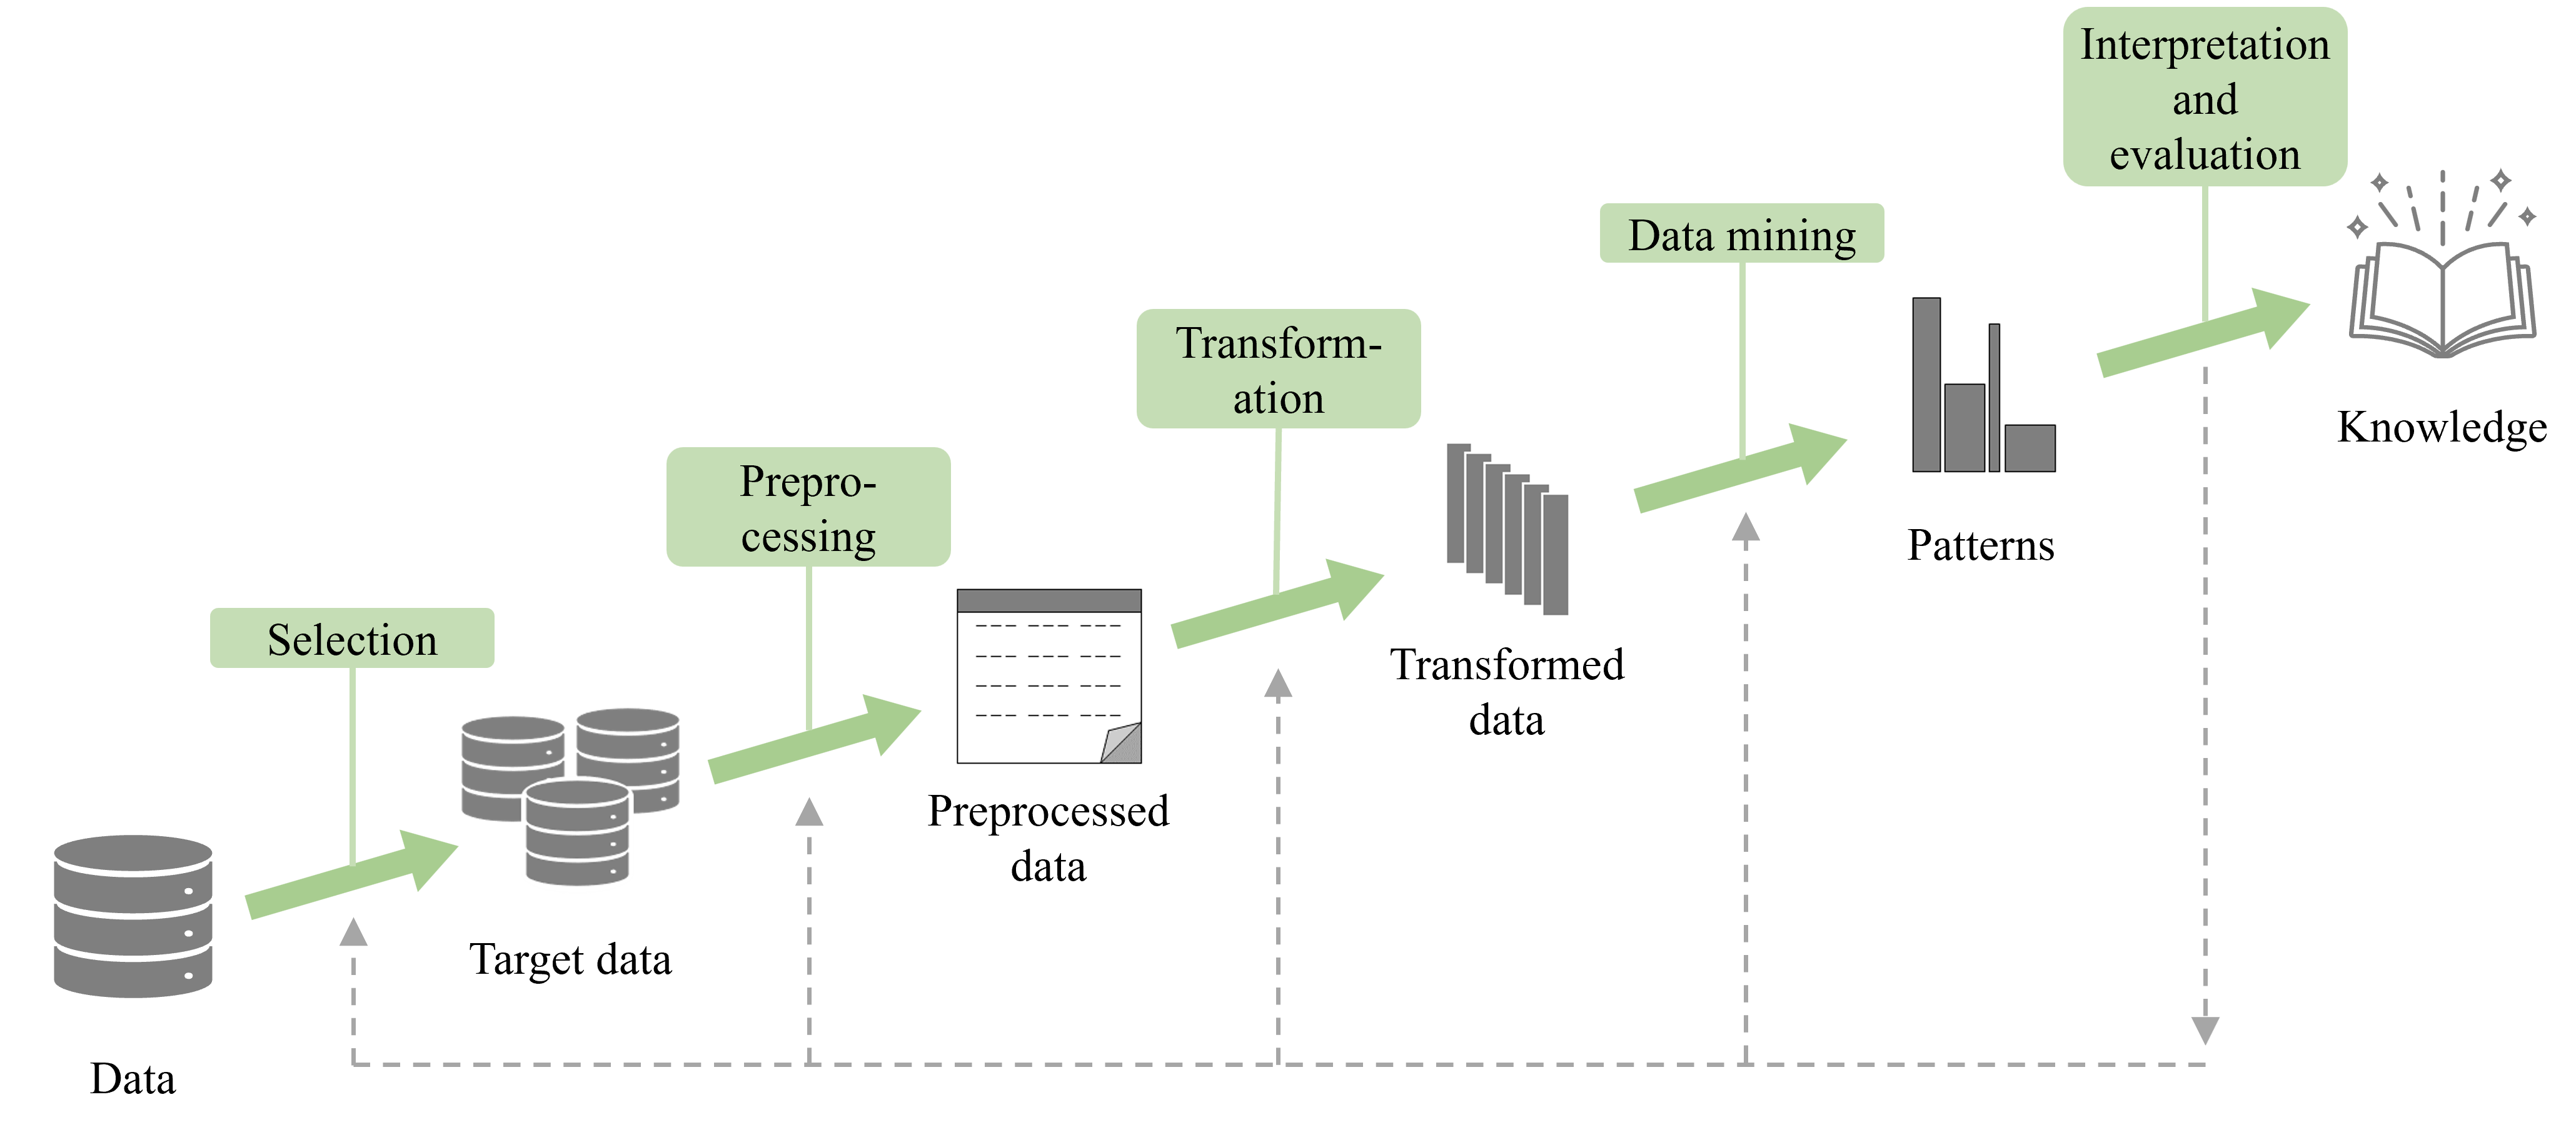
\includegraphics[width=\textwidth]{assets/basics/kdd.png}
  \caption{KDD process}
  \label{fig:1_kdd}
\end{figure}

The next process model is specifically developed for \textbf{L* lifecycle model}\sidenote{L* lifecycle model} with multiple stages as shown in \ref{fig:1_l_star}. 

\begin{figure}[H]
  \centering
  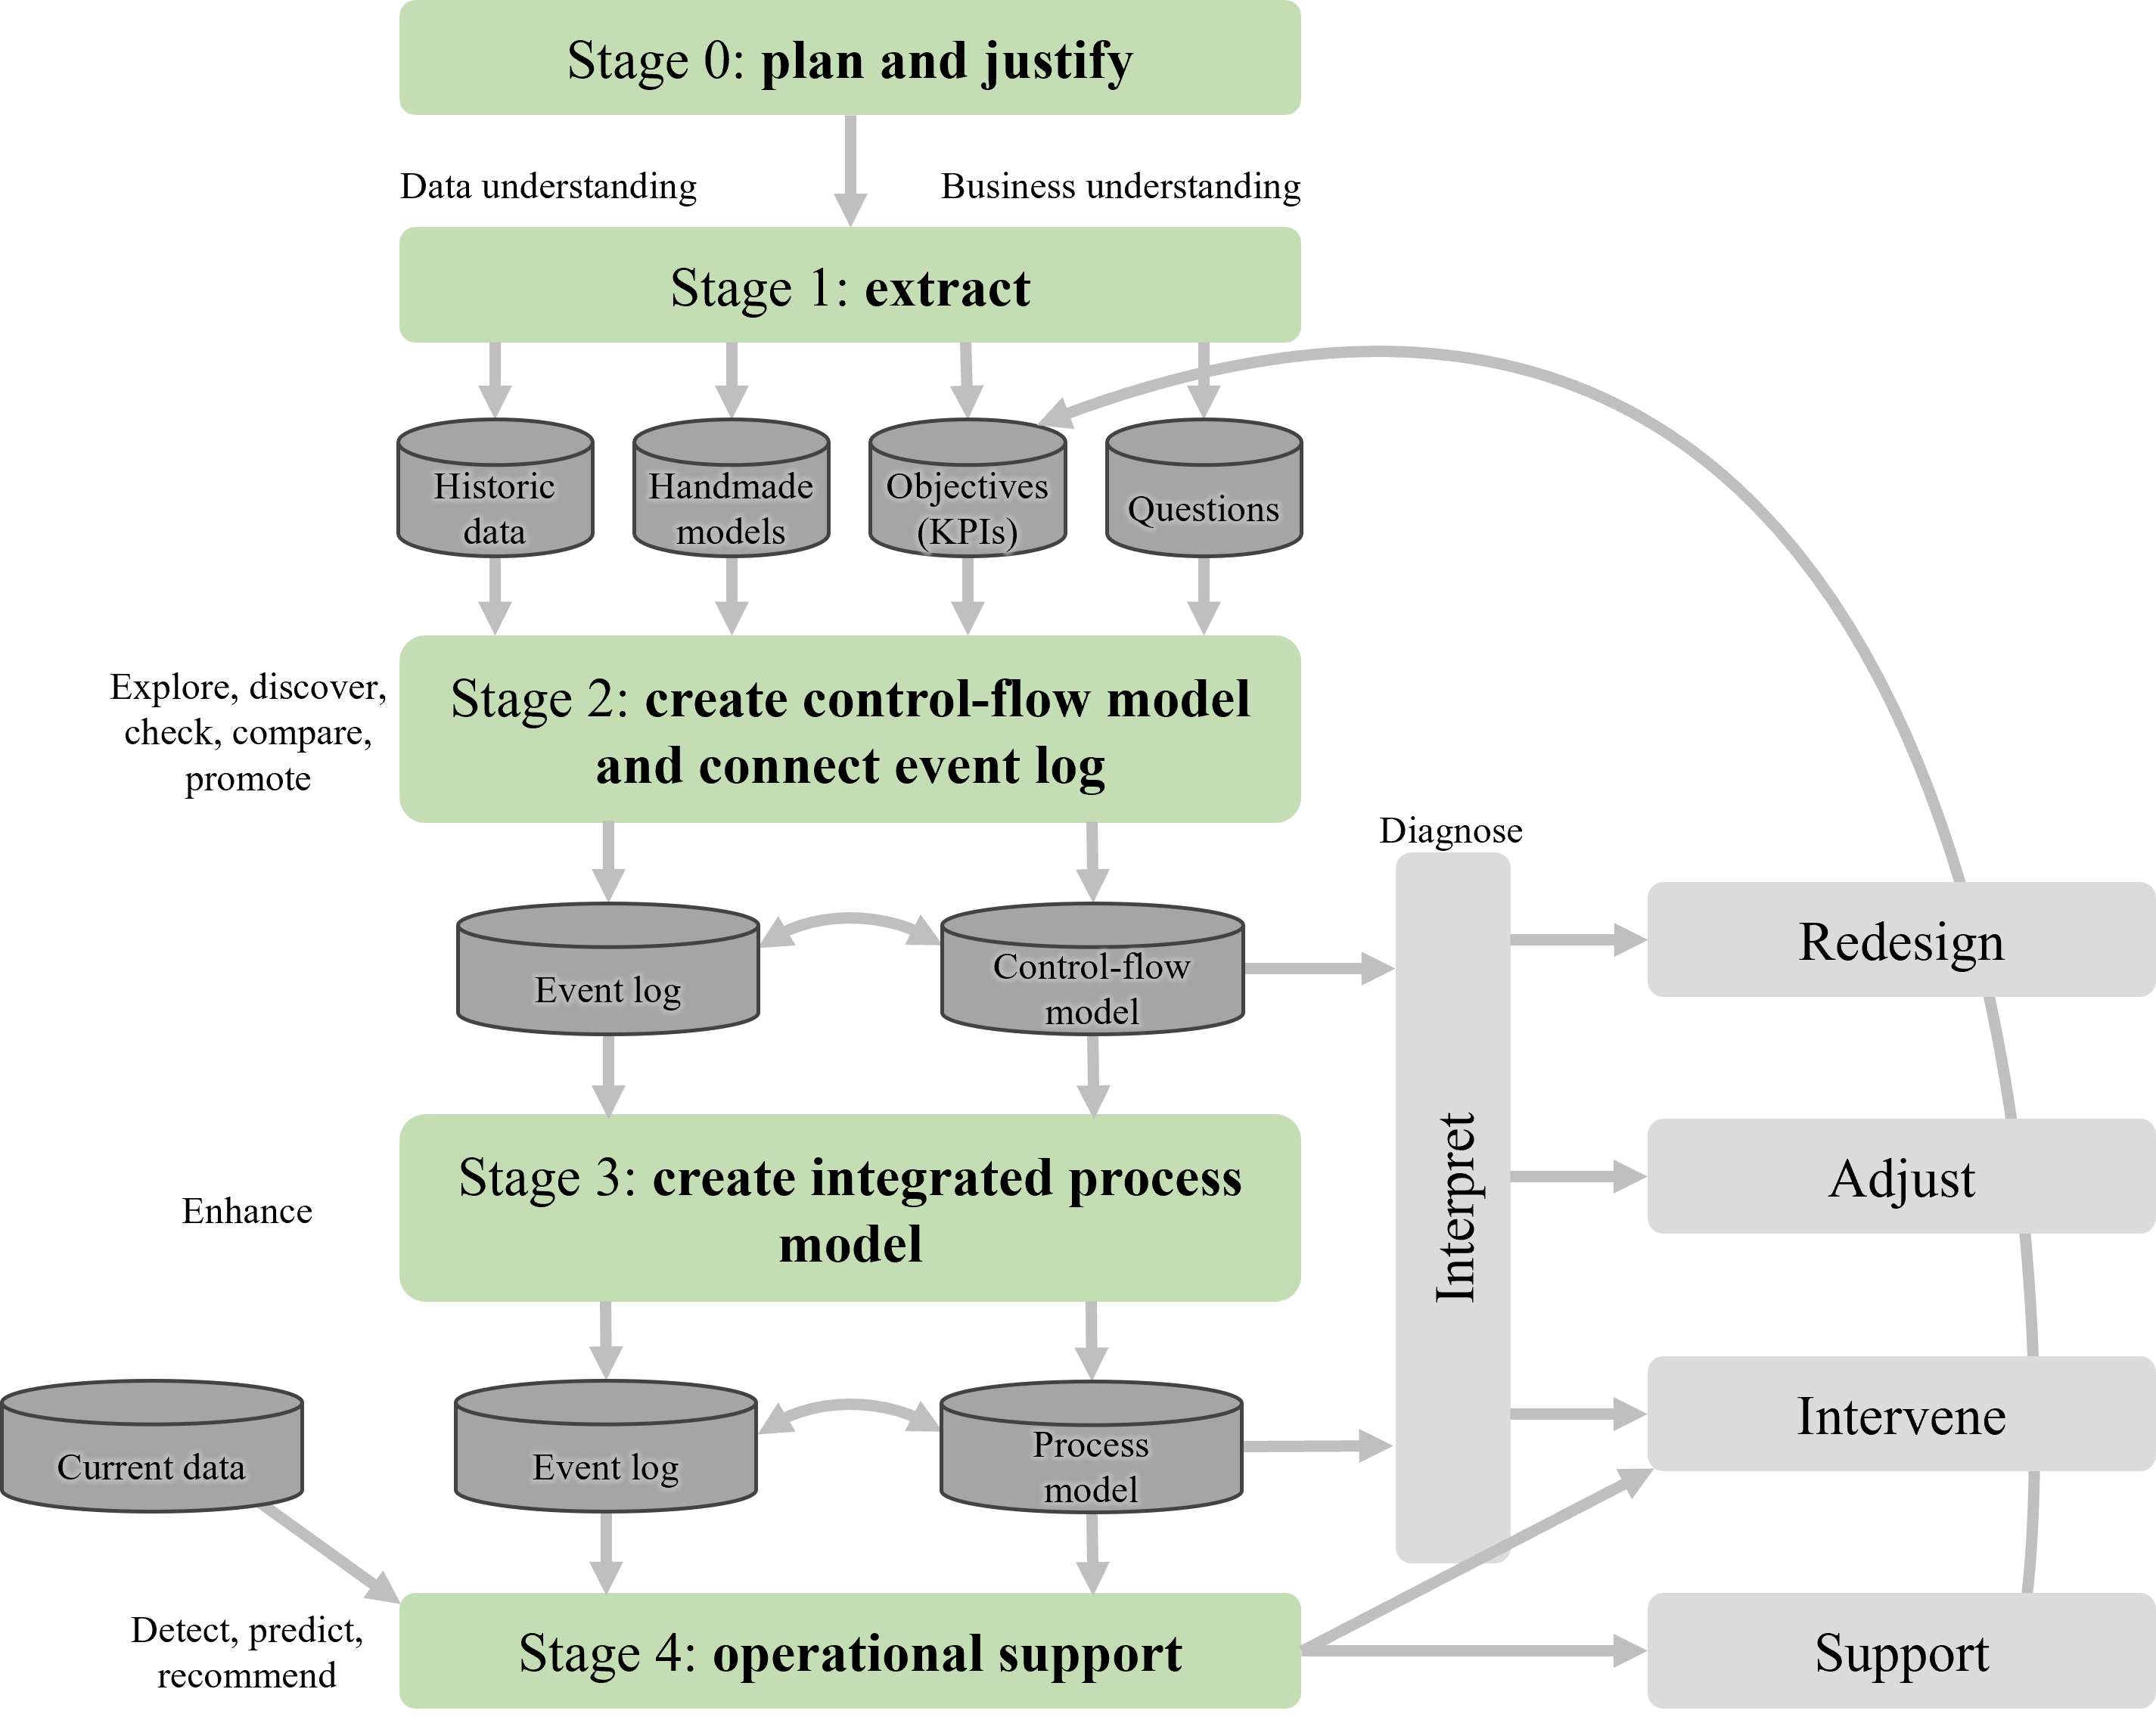
\includegraphics[width=0.7\textwidth]{assets/basics/l_star.png}
  \caption{L* lifecycle model}
  \label{fig:1_l_star}
\end{figure}

Furthermore, we have two methodologies the process model can be related to. Important to implement and solidify are improvements in both.
\begin{itemize}
  \item \textbf{PDCA}\sidenote{PDCA} stands for Plan-Do-Check-Act and is a never-ending cycle with exactly these steps. 
  \item The other one \textbf{DMAIC}\sidenote{DMAIC} stands for Define-Measure-Analyze-Improve-Control, with the following subtasks:
  \begin{itemize}
    \item {\color{gray}\footnotesize Define: launch team, establish charter, plan project, gather VOC/VOB, plan for change}
    \item {\color{gray}\footnotesize Measure: document process, collect baseline data, narrow project focus}
    \item {\color{gray}\footnotesize Analyze: analyze data, identify root causes, identify and remove waste}
    \item {\color{gray}\footnotesize Improve: generate, evaluate, and optimize solutions, pilot, plan and implement}
    \item {\color{gray}\footnotesize Control: control the process, validate project benefits}
  \end{itemize}
\end{itemize}

Finally, we have two processes with the same components, but different ordering of the steps as can be seen in \ref{fig:1_etl_and_elt}. The short terms for the processes are \textbf{ETL}\sidenote{ETL} (extract, transform, load) and \textbf{ELT}\sidenote{ELT} (extract, load, transform).

\begin{figure}[H]
  \centering

  \subcaptionbox{ETL with data warehouse}{
    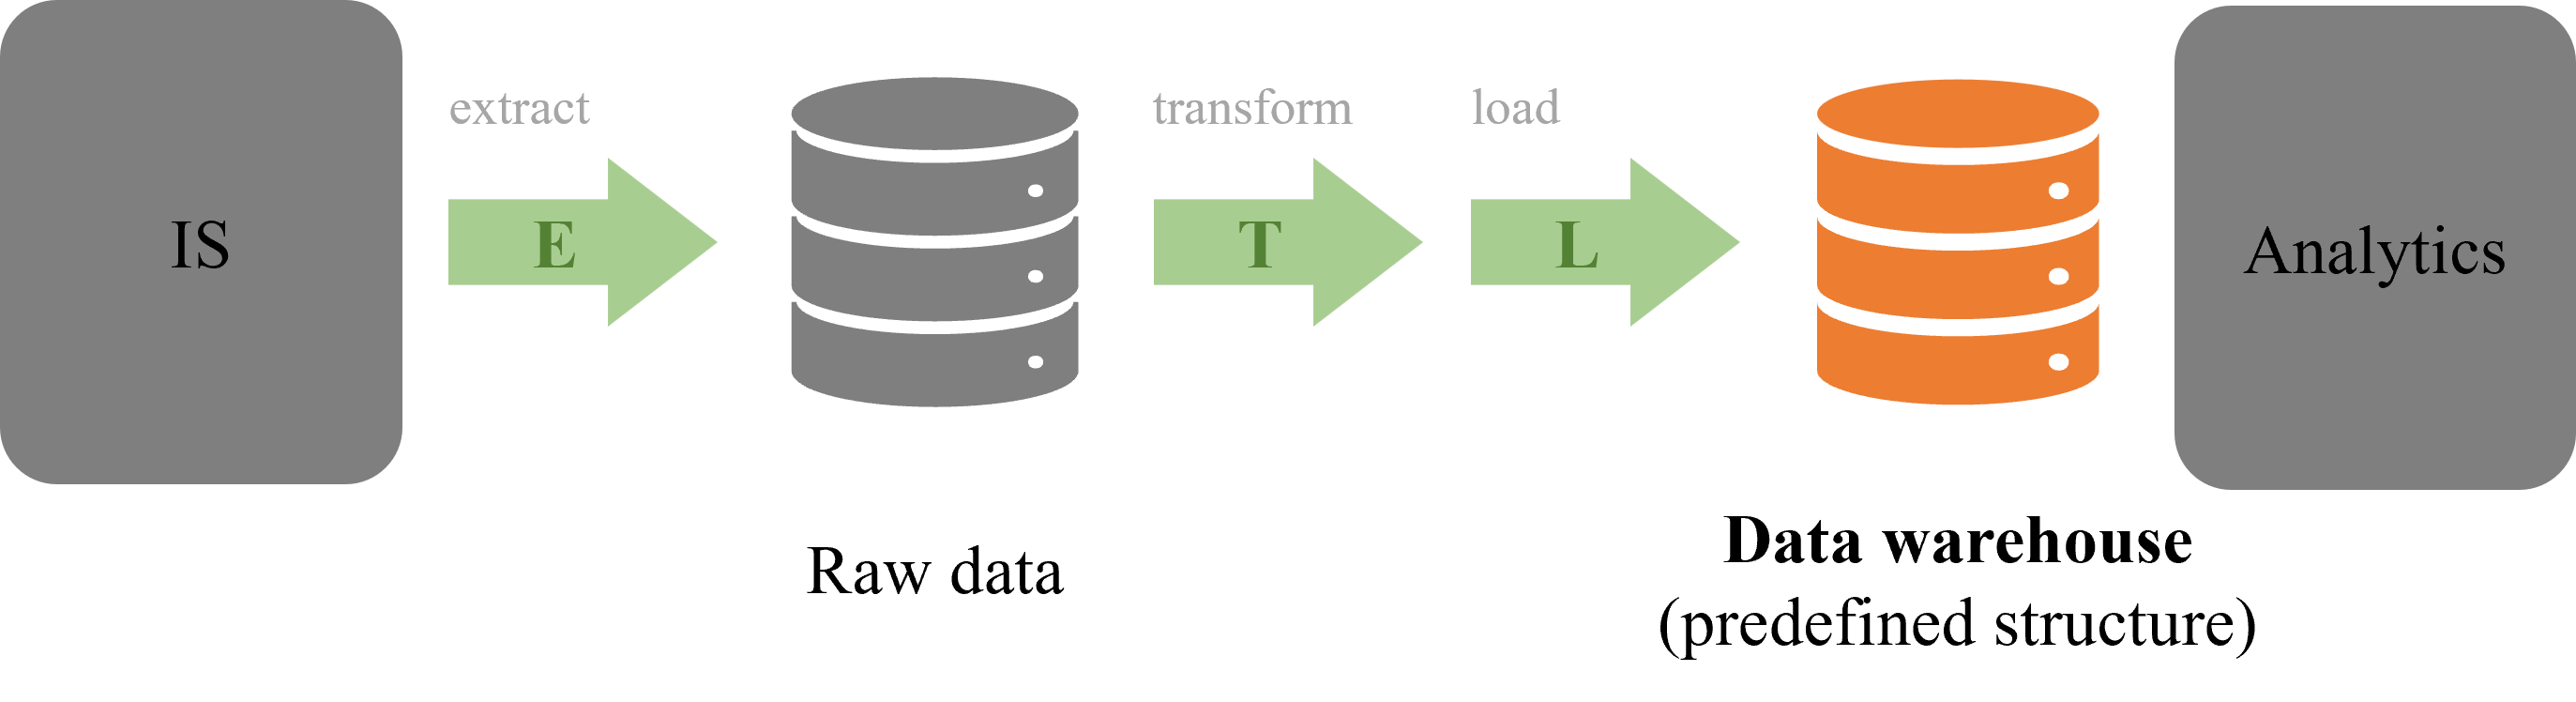
\includegraphics[width=0.45\textwidth]{assets/basics/etl.png}
  }
  \\\vspace*{0.5cm}
  \subcaptionbox{ELT with data lake}{
    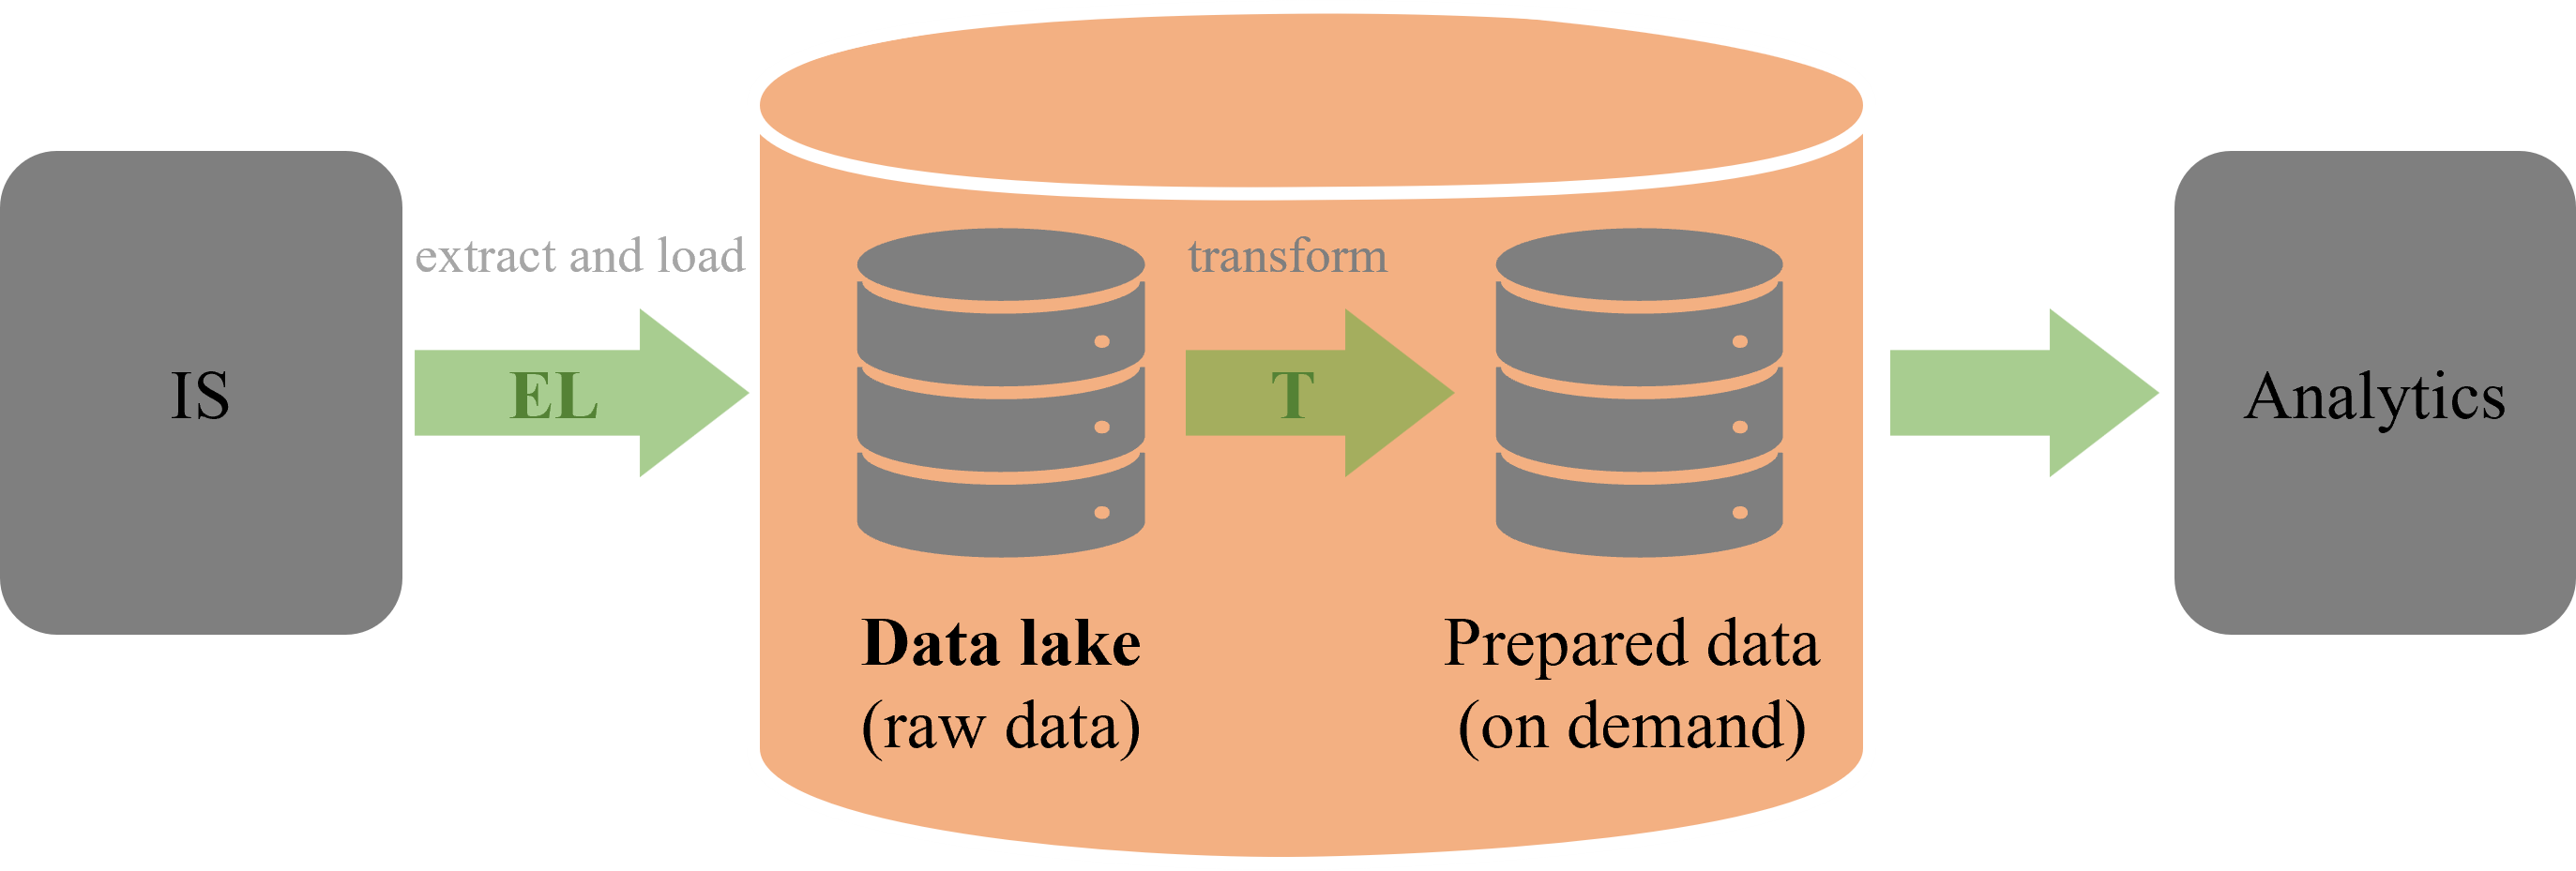
\includegraphics[width=0.45\textwidth]{assets/basics/elt.png}
  }

  \caption{Processes with extraction, transform, and load steps}
  \label{fig:1_etl_and_elt}
\end{figure}

As a final note on which steps are usually the most time-expensive: there is a so-called "80/20 rule" stating:
\begin{itemize}
  \item 80\% of a data scientist's time is spent on finding, cleaning, preprocessing, and organizing data. This leaves only 20\% to actually perform an analysis.
  \item On the other hand, we have 20\% effort determining 80\% of the final result.
\end{itemize}

\begin{figure}[H]
  \centering
  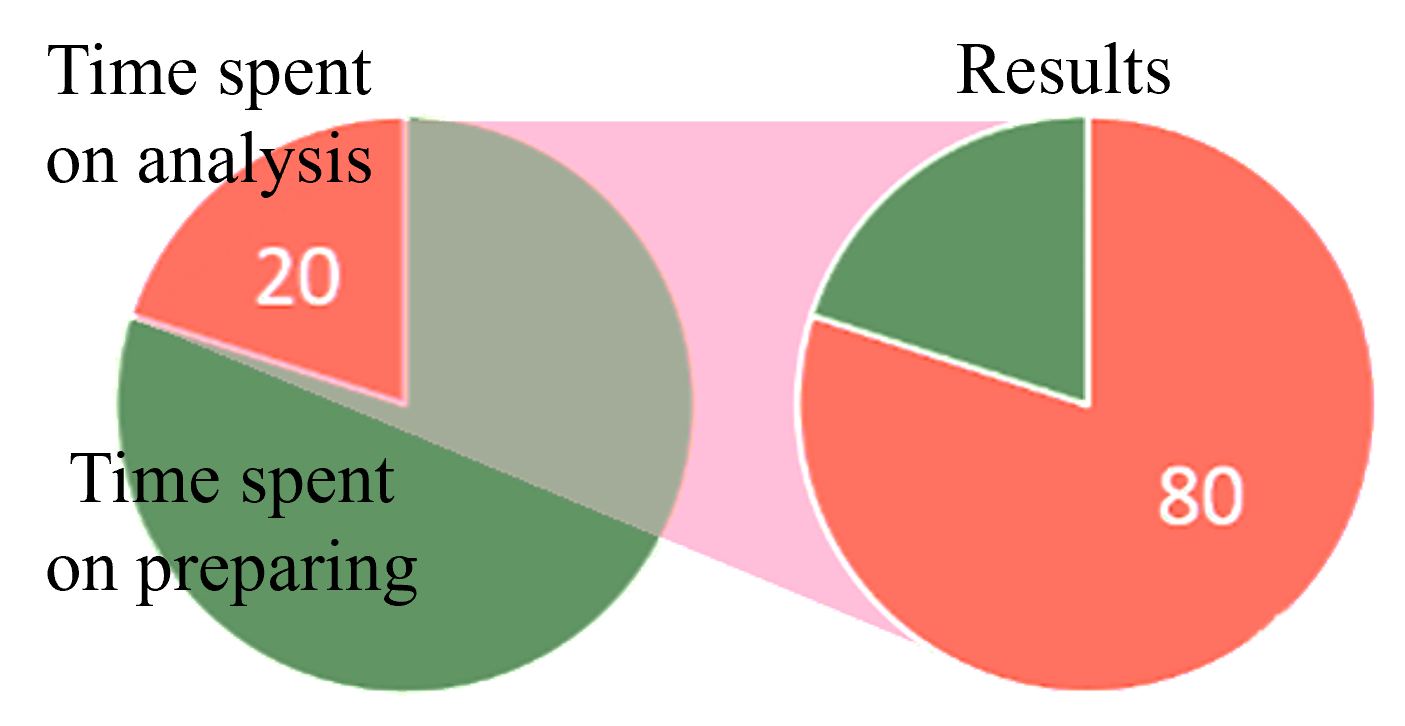
\includegraphics[width=0.4\textwidth]{assets/basics/80_20.png}
  \caption{80-20 rule}
  \label{fig:1_80_20}
\end{figure}